\documentclass[12pt,letter]{article}
\usepackage{../downey_format}

\begin{document}
	
	% set the section number, along with figure and equation numbers
	\setcounter{section}{8}	
	\setcounter{figure}{0}   
	\renewcommand\thefigure{\thesection.\arabic{figure}}
	\setcounter{equation}{0}   
	\renewcommand\theequation{\thesection.\arabic{equation}}

	\section{Experimental Vibrations}
	
Experimental vibration testing requires the practitioner to understand the basics of testing hardware and digital signal processing.


\begin{vibration_case_study}

	On August 14, 2018, the Ponte Morandi viaduct in Genoa Italy collapsed, killing 43 and displacing hundreds of people from their homes. The Morandi viaduct was a cable-stayed bridge with uniquely few stays, typically only two per span. The Stays were a hybrid of steel cables overlaid with concrete. The concrete overlay made the direct inspection of the stays impossible. 
	
	While the exact cause may never be known, is suspected that one of the stay cables within the concrete failed due to corrosion and poor maintenance causing a bridge with very little redundancy in its design to fail\protect\footnotemark[1].
	
	In 2017, researchers from the Polytechnic University of Milan instrumented and studied the vibration characteristics of the bridge and noted that the modal frequencies of the stays on pillar 9 (the one that collapsed) were more than 10\% different than other stays on the bridge. While it's always hard to draw conclusions from one test, comparing modal frequencies between two similar structures can be useful for tracking damage. 
 
	\begin{figure}[H]
		\centering
		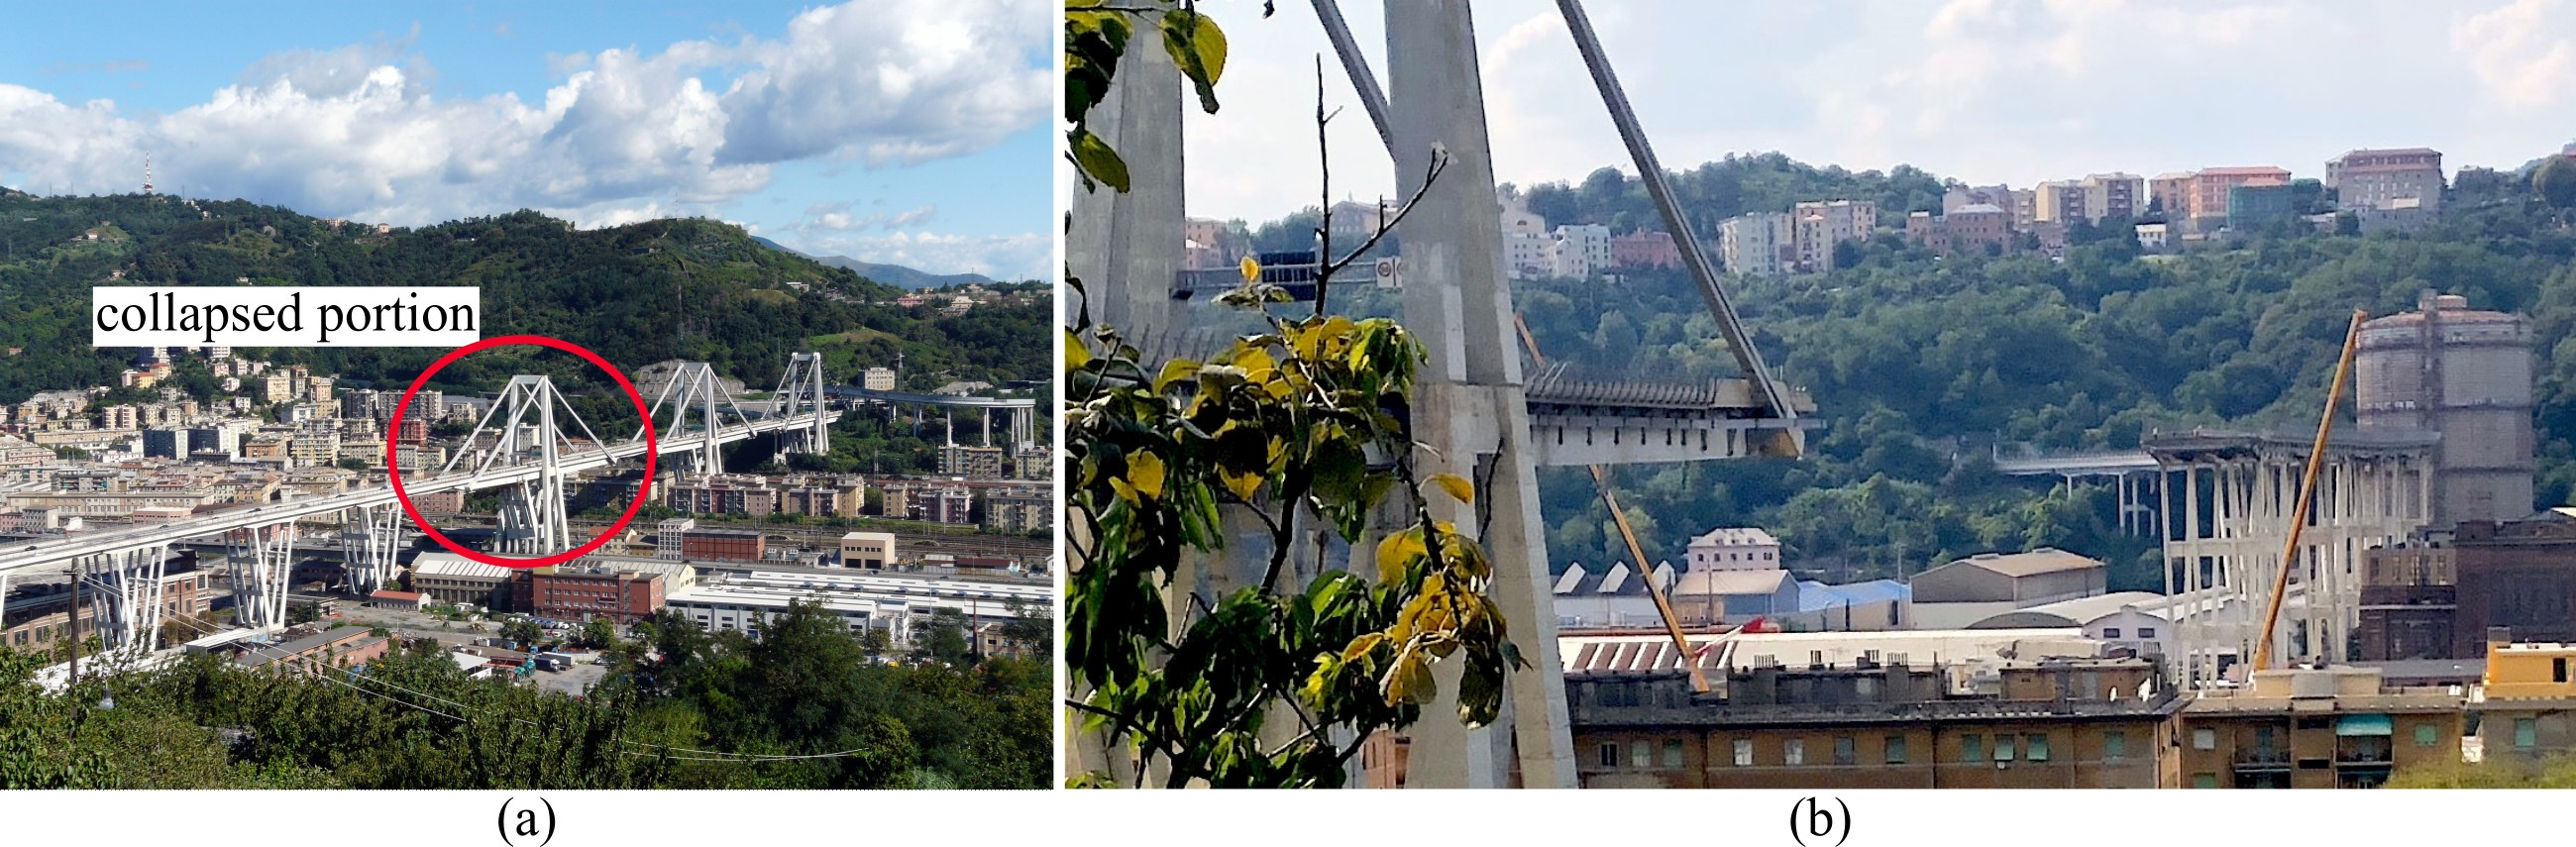
\includegraphics[width=6in]{../figures/ponte_morandi_bridge}
		\caption{The Ponte Morandi bridge, showing the bridge: a) before the collapse\protect\footnotemark[2], and; b) after collapse\protect\footnotemark[3]. }
	\end{figure}
		
	\footnotetext[1]{Rymsza, Janusz. ``Causes of the Collapse of the Polcevera Viaduct in Genoa, Italy.'' Applied Sciences 11, no. 17 (2021): 8098. https://doi.org/10.3390/app11178098.} 	
	\footnotetext[2]{Davide Papalini, CC BY-SA 3.0 $<$https://creativecommons.org/licenses/by-sa/3.0$>$, via Wikimedia Commons} 
	\footnotetext[3]{Michele Ferraris, CC BY-SA 4.0 $<$https://creativecommons.org/licenses/by-sa/4.0$>$, via Wikimedia Commons} 
\end{vibration_case_study}
		
		
\subsection{Hardware for vibration testing}

The measurement of vibrating systems requires specialized hardware. While a variety of vendors sell vibration measurement systems in a number of form factors, the general hardware requirements remain constant. To study the dynamic response of systems subjected to a wide range of excitation, the basic hardware requirements are: \emph{Exciter} - A system to provide a measurable input to the system, \emph{Transducers} - Sensors used for converting the mechanical movements of the structure, and \emph{data acquisition} - Hardware for digitizing the signal generated by the transducers.

\begin{figure}[H]
	\centering
	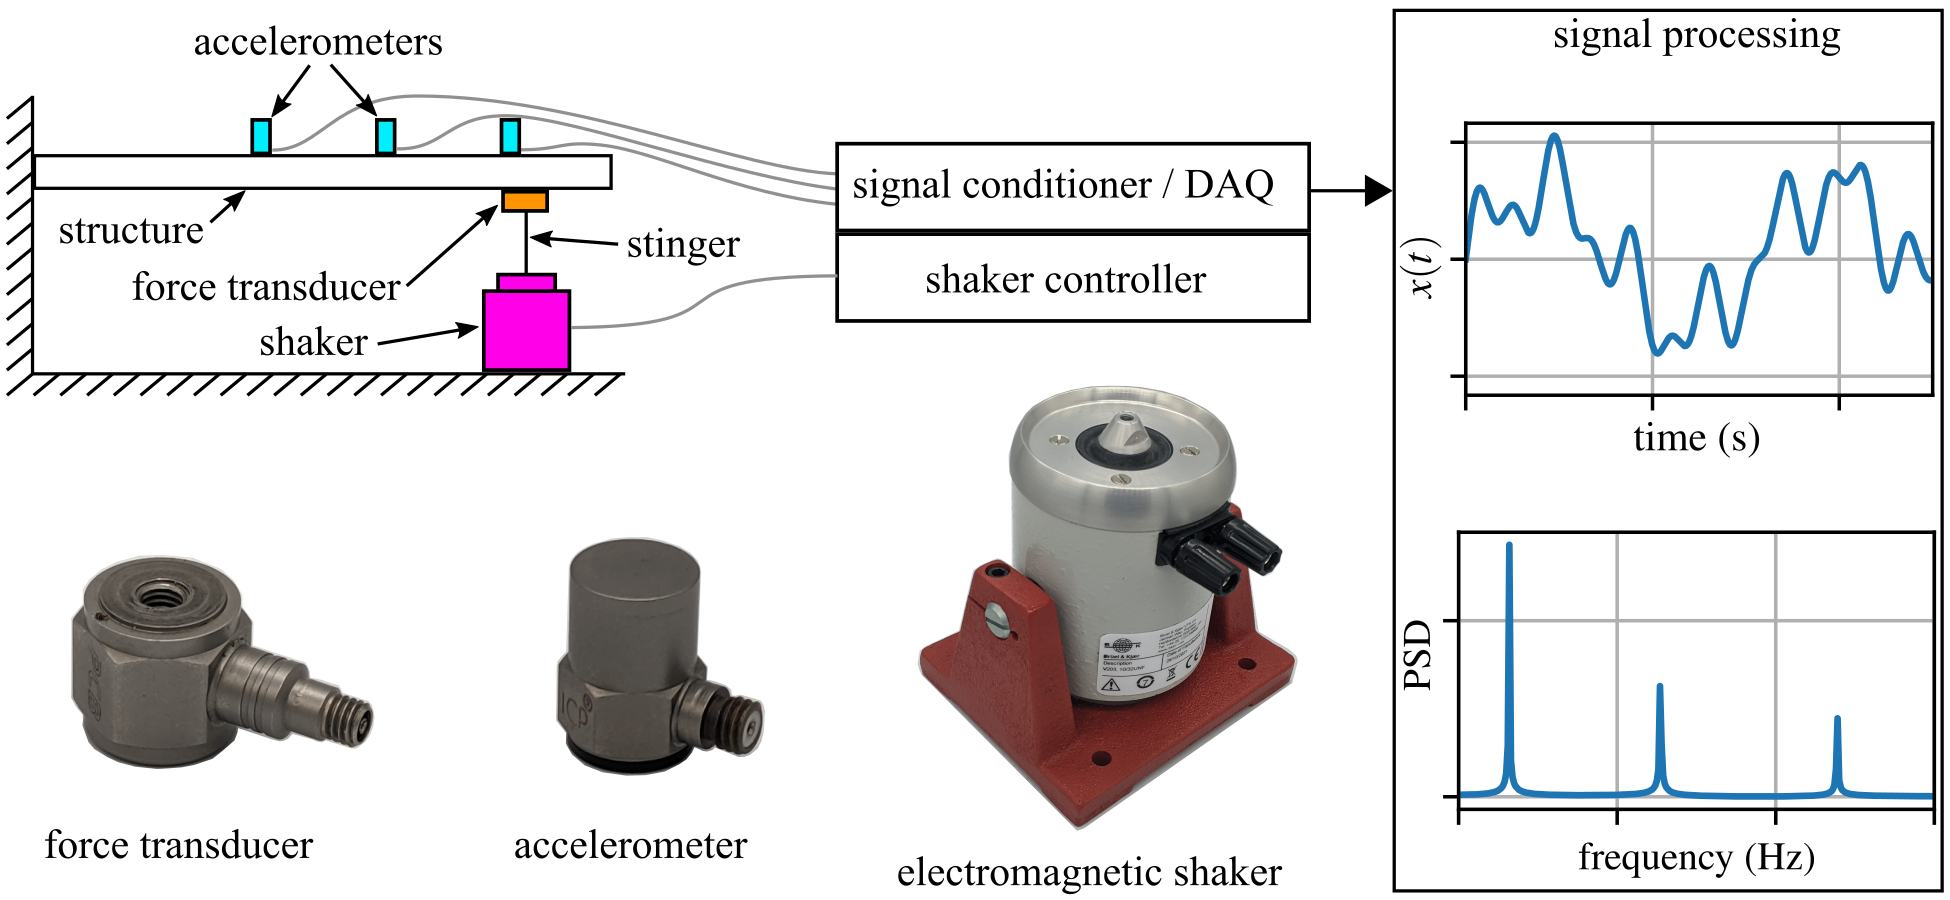
\includegraphics[]{../figures/vibration_testing.png}
	\caption{Key components for performing experimental modal analysis.}
	\label{fig:vibration_testing}
\end{figure} 




 

\begin{figure}[H]
    \centering
    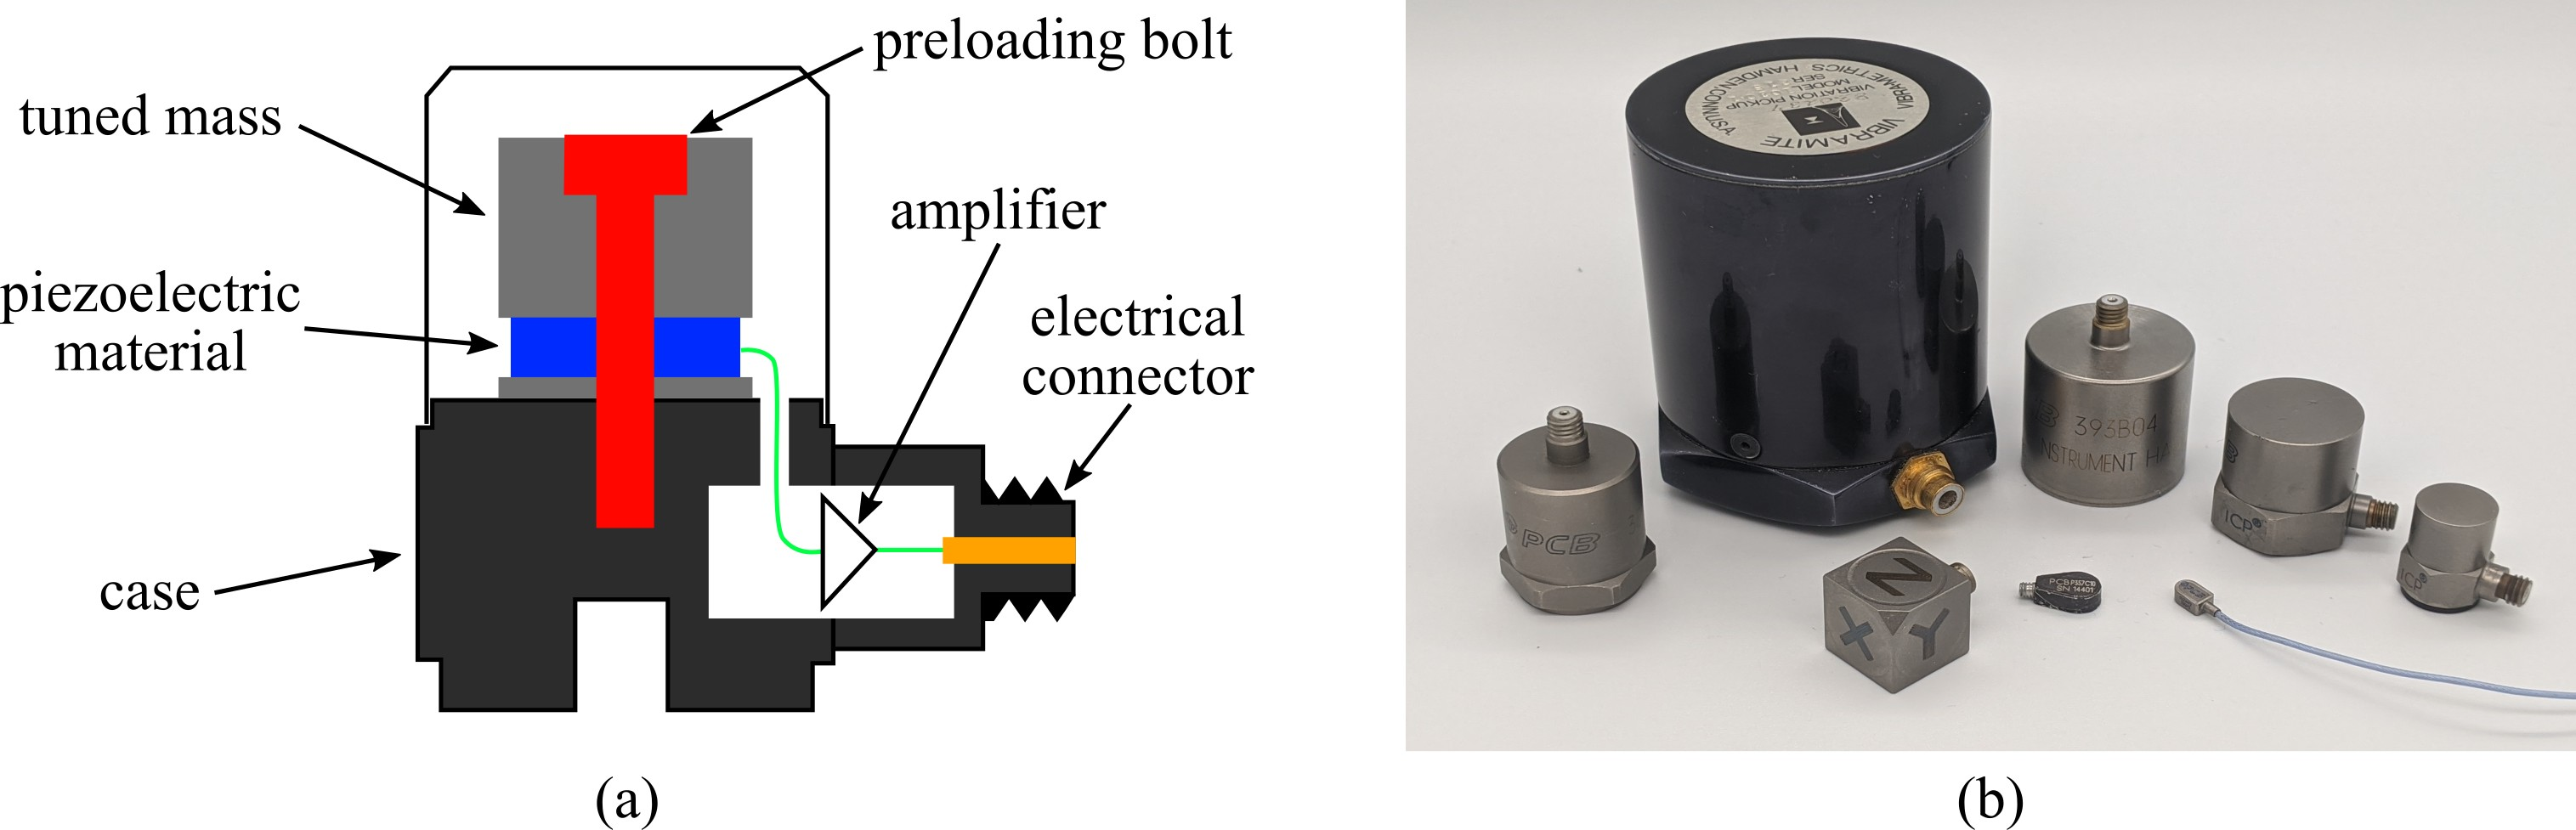
\includegraphics[width=6.5in]{../figures/accelerometers}
    \caption{Integrated Electronics Piezo-Electric (IEPE) accelerometers, showing: (a) the cross-section of a typical IEPE) accelerometer with key components annotated, and; (b) selection of IEPE accelerometers for various applications.}
    \label{fig:accelerometers}
\end{figure} 








\begin{table}[H]
\caption{Parameters for various IEPE accelerometers.}
\resizebox{\textwidth}{!}{\begin{tabular}{@{}llllll@{}}
\toprule
\multicolumn{1}{c}{parameter} & \multicolumn{5}{c}{accelerometers} \\ \midrule
model number & PCB 393B31 & PCB  393B04 & PCB 352C67 & PCB 352A21 & PCB 352A92 \\
Sensitivity($\pm$ 10 \%) & 10.0 V/g & 1000 mV/g & 100 mV/g & 10 mV/g & 0.25 mV/g \\
Measurement Range & $\pm$ 0.5 g pk & $\pm$ 5 g pk & $\pm$ 50 g pk & $\pm$ 500 g pk & $\pm$ 20 kg pk \\
Frequency Range($\pm$ 5 \%) & 0.1 to 200 Hz & 0.06 to 450 Hz & 0.5 to 10 kHz & 1.0 to 10 kHz & 1.2 to 10 kHz \\
Resonant Frequency & \textgreater 700 Hz & \textgreater 2.5 kHz & \textgreater 35 kHz & \textgreater 50 kHz & \textgreater 100 kHz \\
Non-Linearity & $\le$1\% & $\le$1\% & $\le$1\% & $\le$1\% &  \\
Transverse Sensitivity & $\le$5\% & $\le$5\% & $\le$5\% & $\le$5 \% &  \\ \bottomrule
\end{tabular}}
\end{table}


\begin{figure}[H]
	\centering
	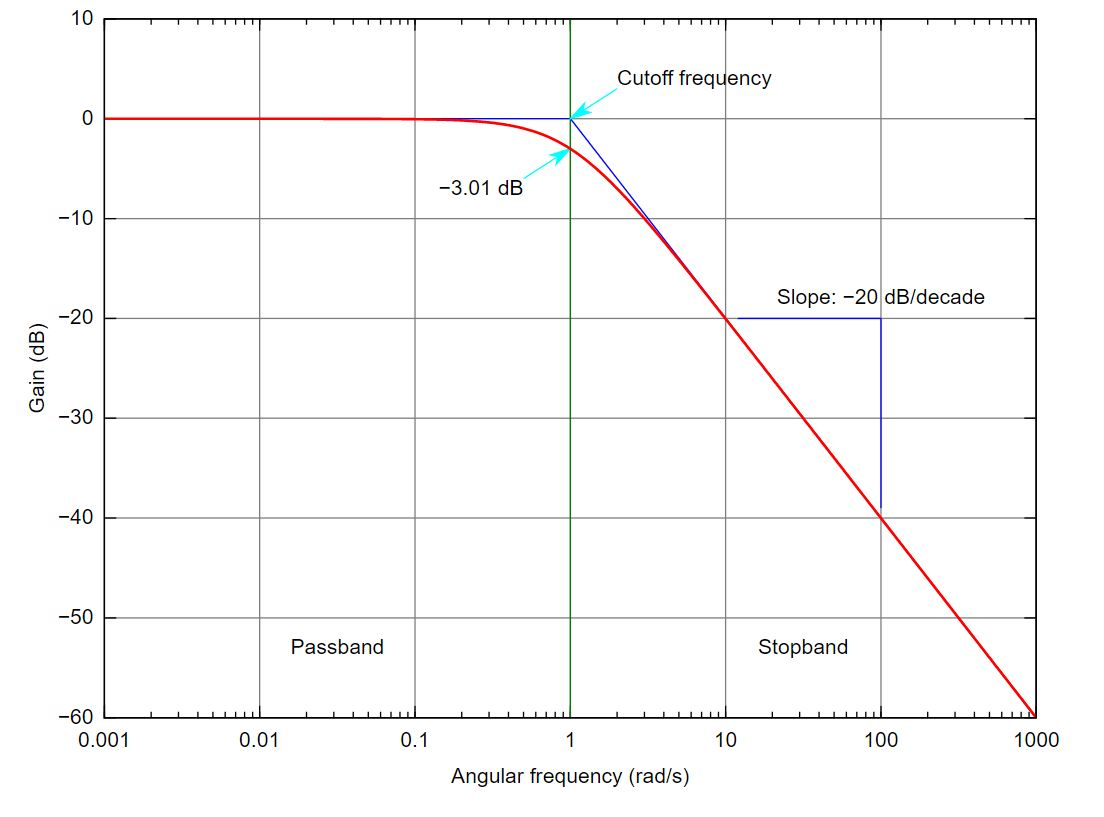
\includegraphics[width=3.5in]{../figures/frequency_rolloff}
	\caption{frequency roll-off.\protect\footnotemark[1] }
	\label{fig:frequency_rolloff}
\end{figure}

\footnotetext[1]{PDerivative work:  KrishnavedalaOriginal:  Omegatron, CC BY-SA 3.0 $<$https://creativecommons.org/licenses/by-sa/3.0$>$, via Wikimedia Commons}






%Measurement Range & 0.5 g pk & \pm 5 g pk & \pm 50 g pk & \pm 100 g pk & \pm 500 g pk & \pm20,000 g pk \\
%Frequency Range(\pm 5 \%) & 0.1 to 200 Hz & 0.06 to 450 Hz & 0.5 to 10,000 Hz & 1 to 5,000 Hz & 1.0 to 10,000 Hz & 1.2 to 10,000 Hz \\


\begin{figure}[H]
    \centering
    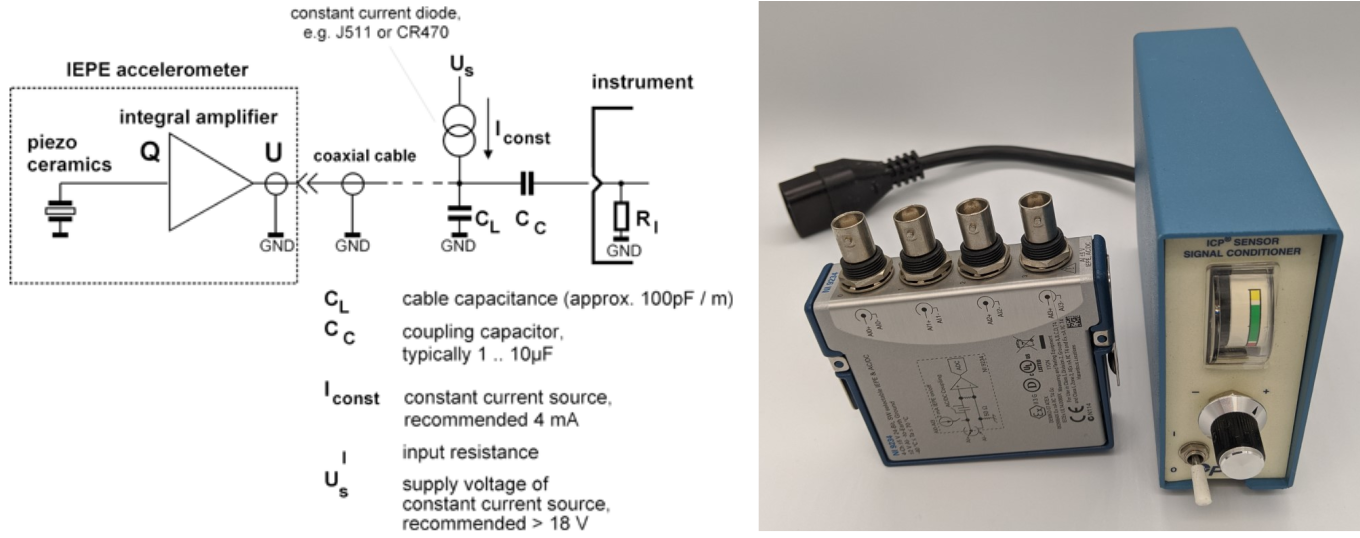
\includegraphics[width=6.5in]{../figures/IEPE.png}
    \caption{Integrated Electronics Piezo-Electric (IEPE)-based measurement system showing the: (a) simplified circuit schematic\protect\footnotemark[1]; and (b) IEPE data acquisition systems in various form factors.}
    \label{fig:IEPE}
\end{figure} 


A modal hammer is used to impart a measured impact into the structure. Figure~\ref{fig:modal_hammer} shows a model hammer with interchangeable tips and the responses generated by the tips. 

\begin{figure}[H]
	\centering
	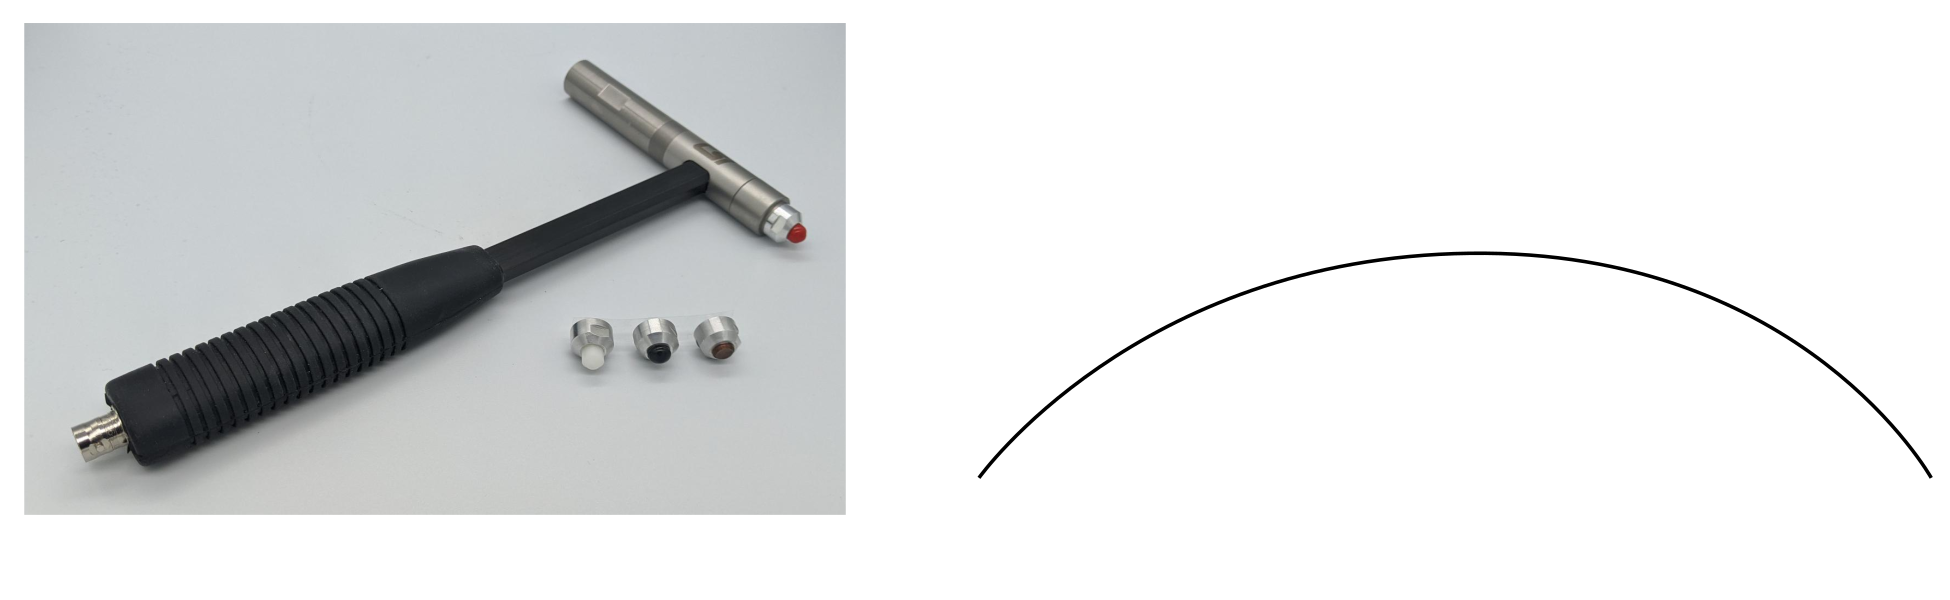
\includegraphics[width=6.5in]{../figures/modal_hammer.png}
	\caption{Model hammer with interchangeable tips.}
	\label{fig:modal_hammer}
\end{figure} 



\footnotetext[1]{``IEPE sensor connected to the input of an instrument'' by JanBurg  CC BY-SA 4.0}  



\pagebreak


\subsection{Digital Signal Processing}


	\begin{review}
	\label{sec:Harry_Nyquist}
		
		Harry Nyquist (February 7, 1889 ? April 4, 1976) was a Swedish physicist and electronic engineer. His parents emigrated to the U.S. in 1907.  He attended the University of North Dakota starting in 1912 where he obtained a B.S. in 1914 and an M.S. in 1915, both in electrical engineering (entry to M.S. was 3 years!). Thereafter, he went to Yale University where he received a Ph.D. in physics in 1917.

		\begin{figure}[H]
			\centering
			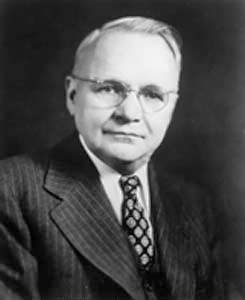
\includegraphics[width=2.71in]{../figures/Harry_Nyquist.jpg}
			\caption{Picture of Harry Nyquist from the American Institute of Physics.\protect\footnotemark[1]}
			\label{fig:Harry_Nyquist}
		\end{figure}
		\footnotetext[1]{Fair use, via Wikimedia Commons}
	\end{review}



\begin{figure}[H]
    \centering
    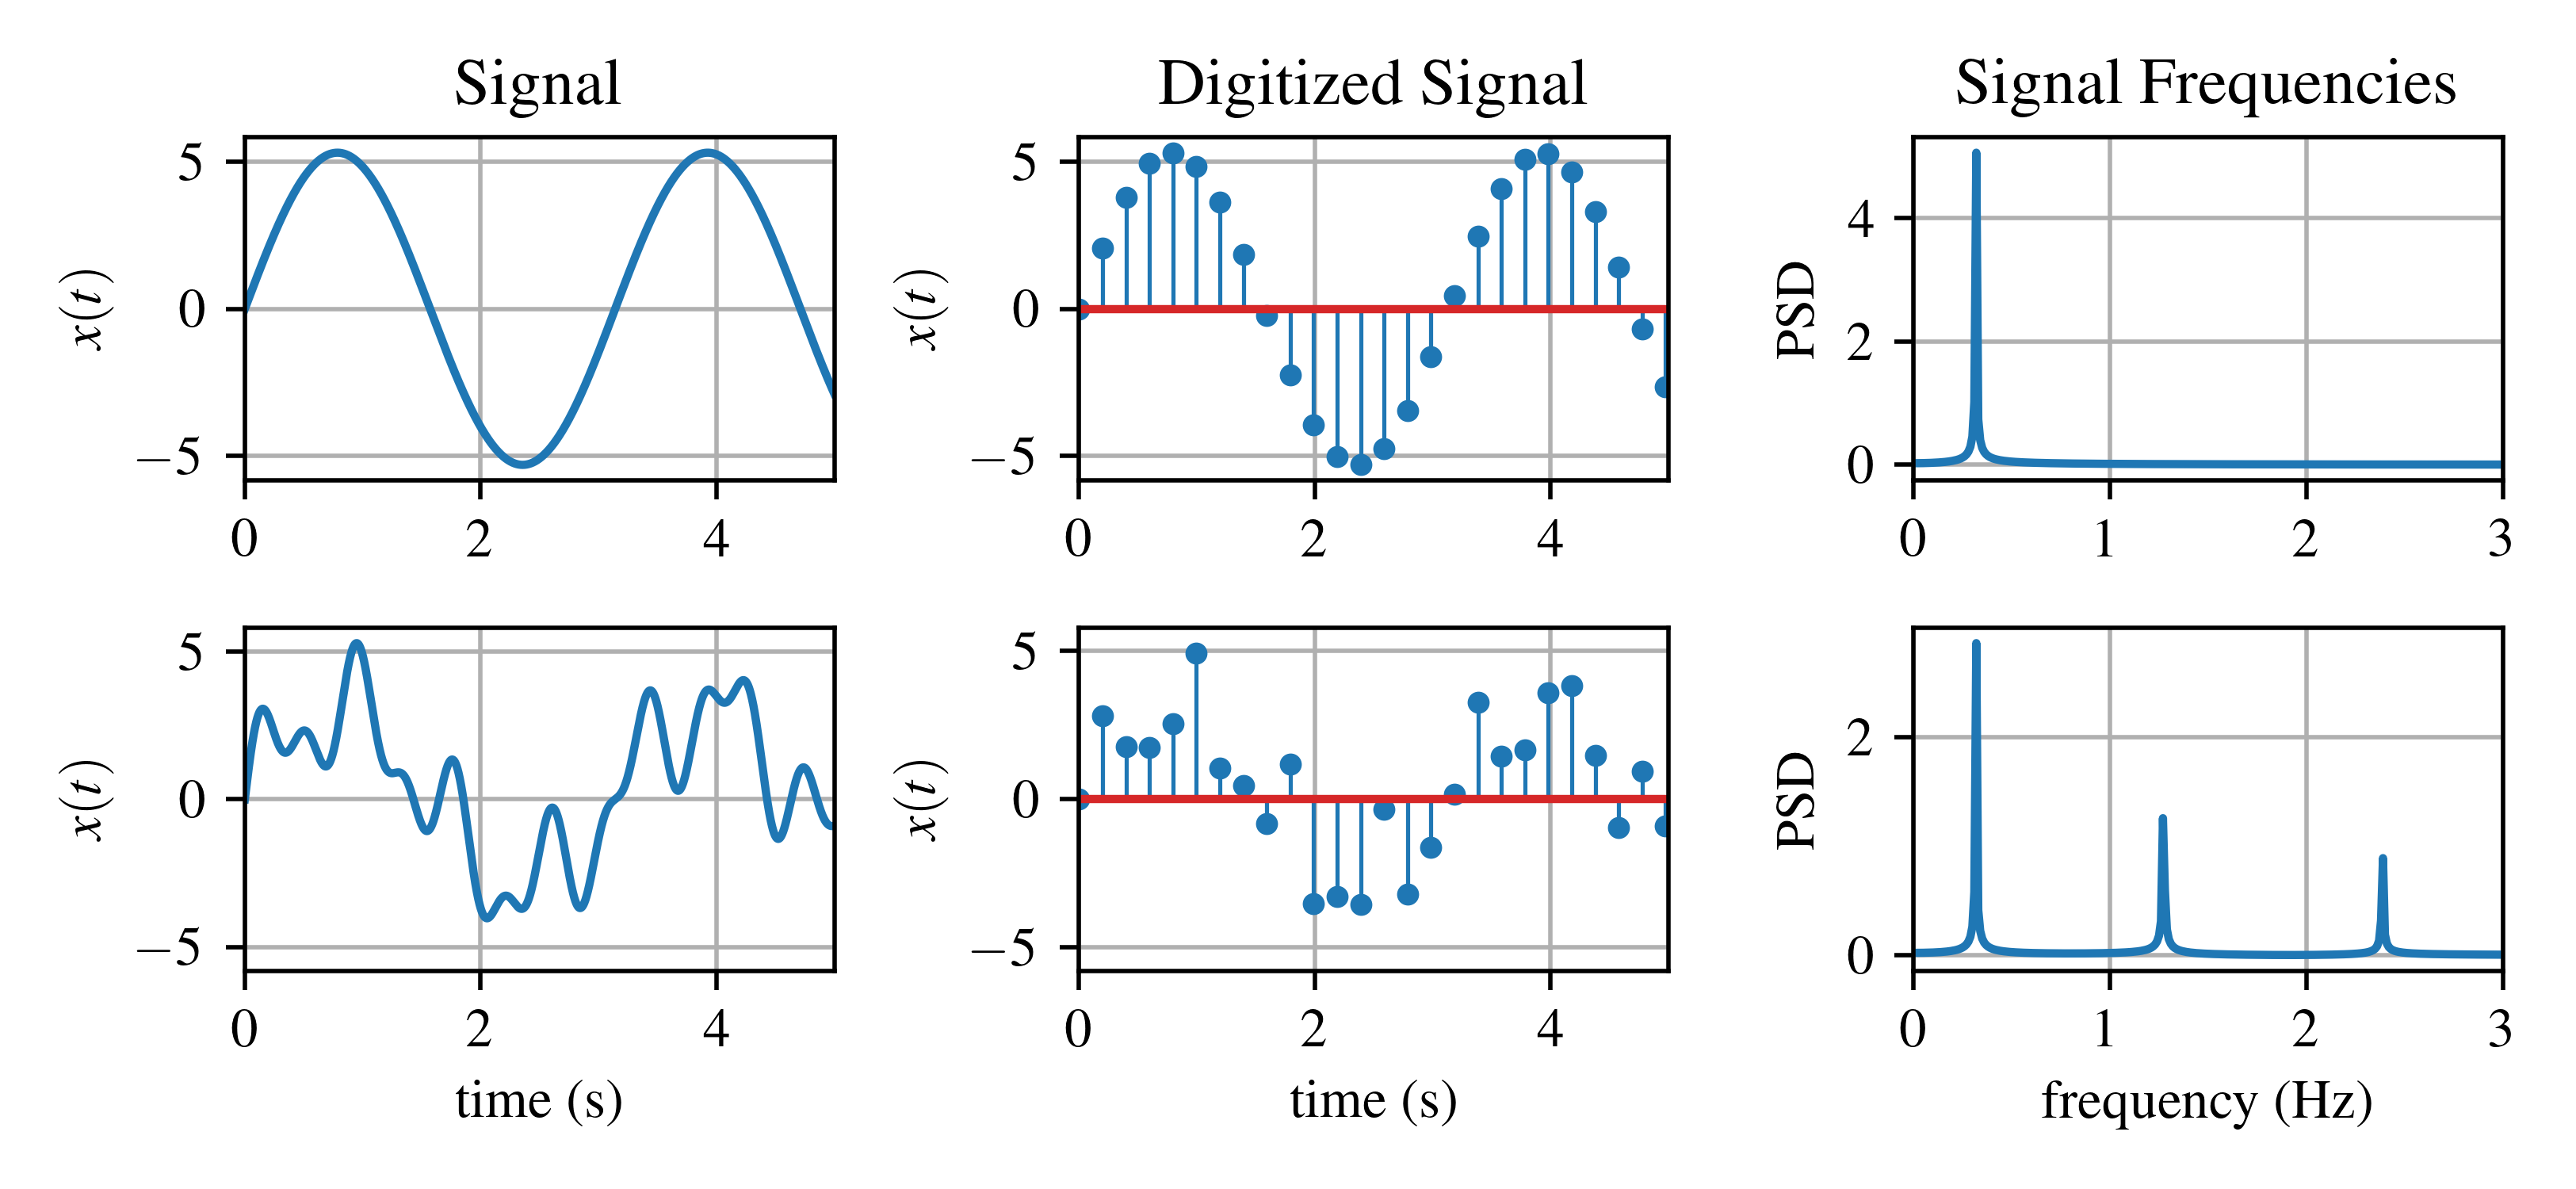
\includegraphics[width=6.5in]{../figures/signal_digitization.png}
    \caption{Digitization of two continuous time-series signals sampled at 5 S/s.}
    \label{fig:signal_digitization}
\end{figure}


The Nyquist-Shannon sampling theorem is a theorem in the field of signal processing that defines the sample rate that permits a discrete sequence of samples (i.e. discrete-time) to sample a continuous-time signal of finite bandwidth. 

\begin{figure}[H]
    \centering
    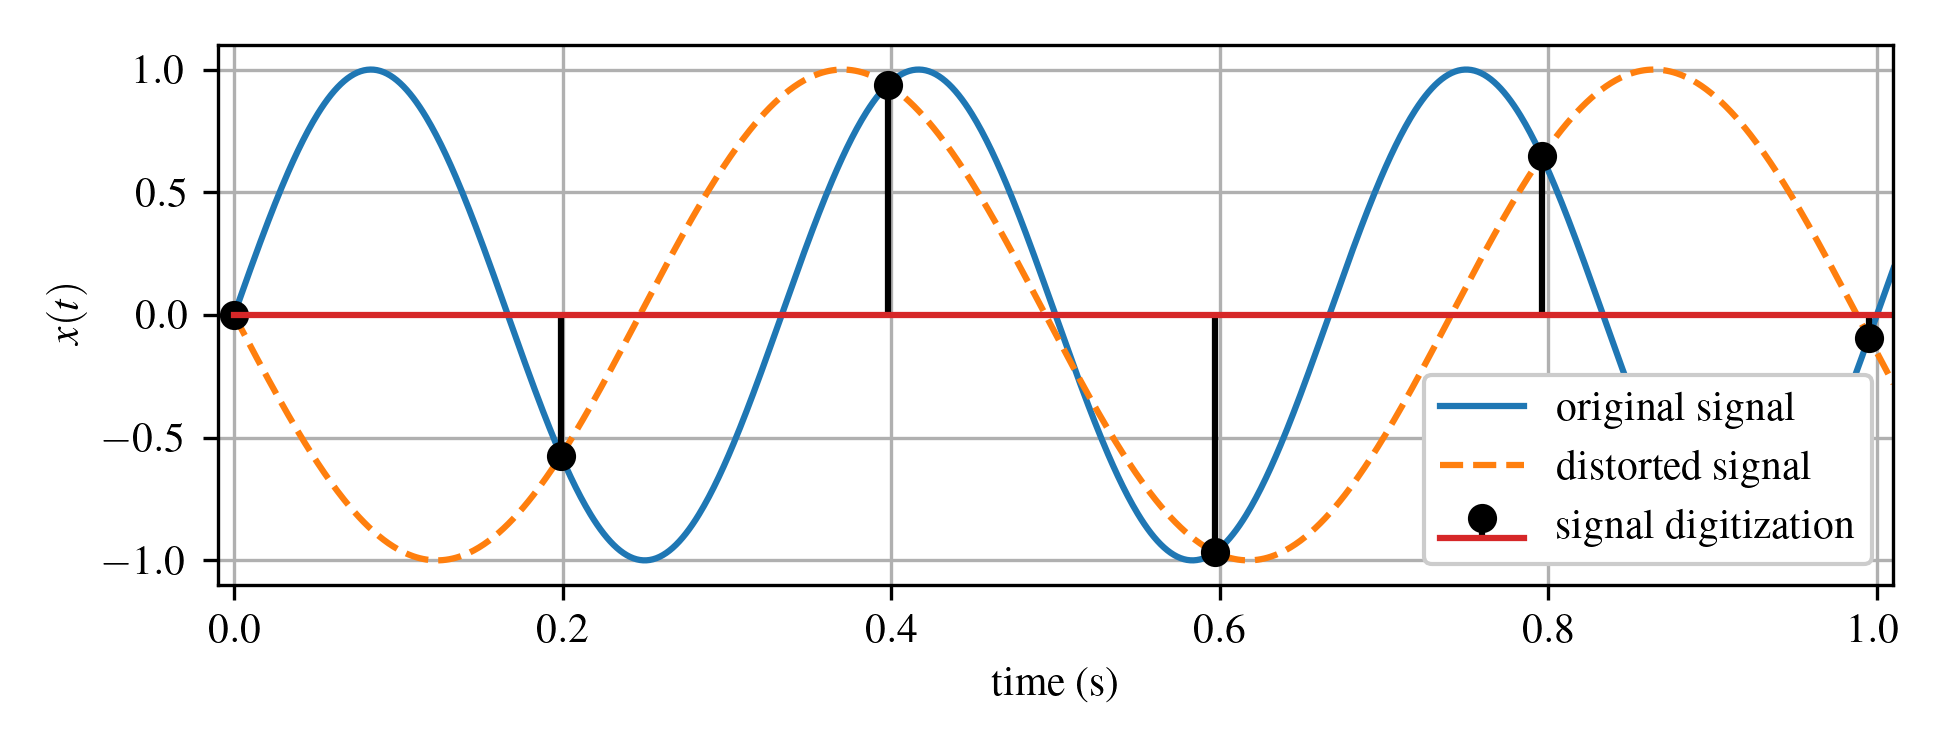
\includegraphics[width=6.5in]{../figures/aliasing.png}
    \caption{Aliasing of a 3 Hz signal that is sampled at 5 S/s.}
    \label{fig:aliasing}
\end{figure}

In signal processing, aliasing is an effect that causes different signals to become indistinguishable from each other.  In this way, the signals become an alias of one another when sampled. Aliasing also accounts for the development of distortion or artifact in a reconstructed signal when compared to the original continuous signal.


\begin{figure}[H]
    \centering
    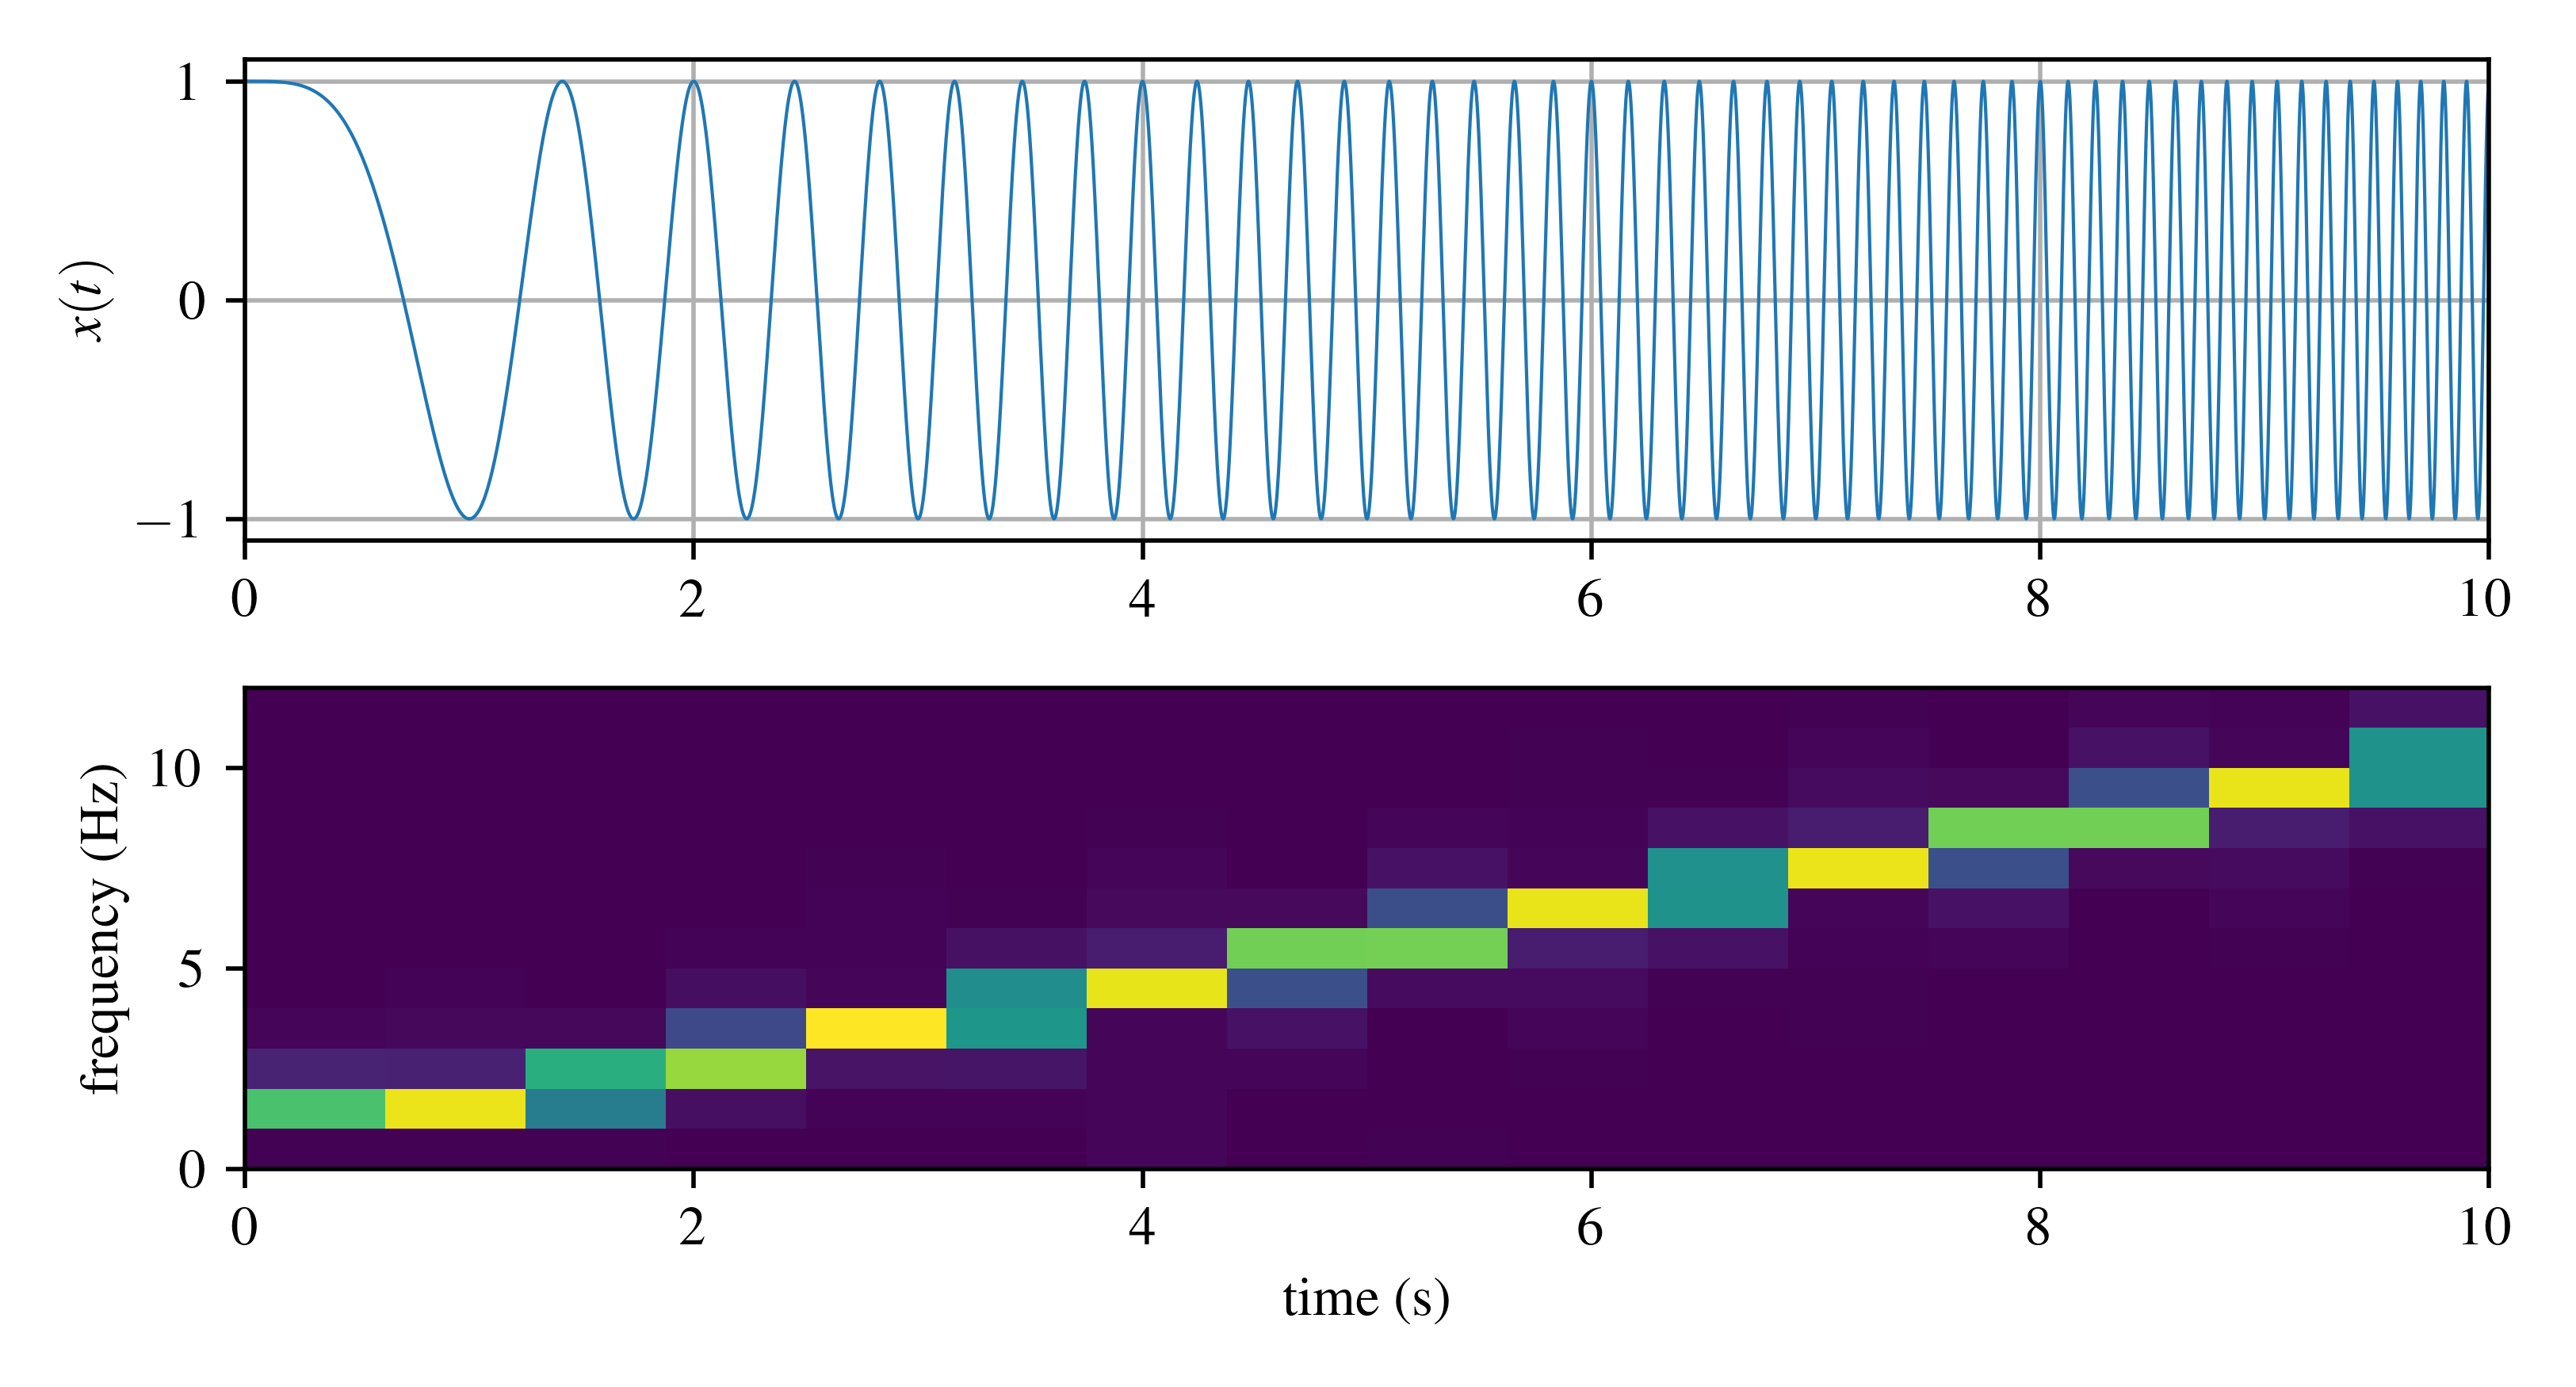
\includegraphics[width=6.5in]{../figures/spectrogram.png}
    \caption{Spectrogram of a 0-10 Hz chirp signal.}
    \label{fig:spectrogram}
\end{figure}

Some of the key parameters in a spectrogram include:

\begin{itemize}
\item window
\item segment length
\item overlap
\end{itemize}


\subsection{Frequency response function}









\end{document}














